\documentclass[tikz]{standalone}

\begin{document}
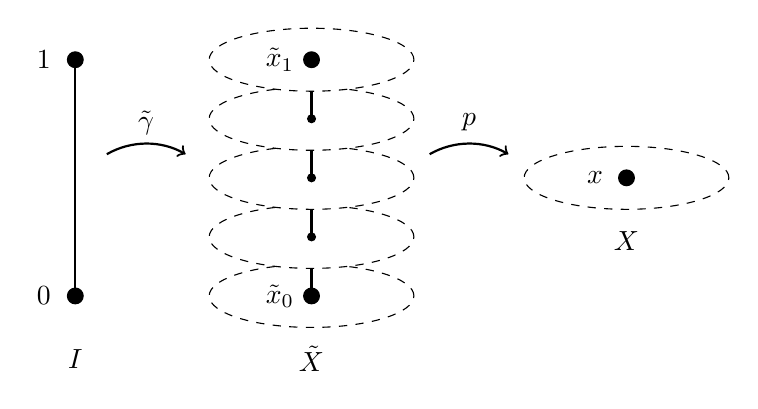
\begin{tikzpicture}

% The interval [0, 1]
\node at (0, -0.8) {$I$};
\draw[thick] (0, 0) -- (0, 3);
\filldraw (0, 0) circle (0.1);
\filldraw (0, 3) circle (0.1);
\node at (-0.4, 0) {$0$};
\node at (-0.4, 3) {$1$};

% A bunch of open sets in \tilde{X}
\node at (3, -0.8) {$\tilde{X}$};
\filldraw[fill=white,draw=black,dashed] (3, 0.00) ellipse (1.3 and 0.4);
\draw[thick] (3, 0.00) -- (3, 0.35);
\filldraw[fill=white,draw=black,dashed] (3, 0.75) ellipse (1.3 and 0.4);
\draw[thick] (3, 0.75) -- (3, 1.10);
\filldraw[fill=white,draw=black,dashed] (3, 1.50) ellipse (1.3 and 0.4);
\draw[thick] (3, 1.50) -- (3, 1.85);
\filldraw[fill=white,draw=black,dashed] (3, 2.25) ellipse (1.3 and 0.4);
\draw[thick] (3, 2.25) -- (3, 2.60);
\filldraw[fill=white,draw=black,dashed] (3, 3.00) ellipse (1.3 and 0.4);
\filldraw (3, 0.00) circle (0.1);
\filldraw (3, 0.75) circle (0.05);
\filldraw (3, 1.50) circle (0.05);
\filldraw (3, 2.25) circle (0.05);
\filldraw (3, 3.00) circle (0.1);
\node at (2.6, 0) {$\tilde{x}_0$};
\node at (2.6, 3) {$\tilde{x}_1$};

% A single open set in X
\node at (7, 0.7) {$X$};
\filldraw[fill=white,draw=black,dashed] (7, 1.5) ellipse (1.3 and 0.4);
\filldraw (7, 1.5) circle (0.1);
\node at (6.6, 1.5) {$x$};

% The path \tilde{\gamma}
\draw[thick,->] (0.4, 1.8) arc (120:60:1);
\node at (0.9, 2.2) {$\tilde{\gamma}$};

% The projection p
\draw[thick,->] (4.5, 1.8) arc (120:60:1);
\node at (5.0, 2.2) {$p$};

\end{tikzpicture}
\end{document}
